\section*{Aufgabe 3 (30 Punkte)}
\vspace{0.4cm}
\subsection*{\frage{1}{4}}
Es sei
\begin{align*}
	s = \sum \limits_{i= 1}^3
	\sum \limits_{j= 1}^2
	\sum \limits_{k= 1}^4
	(i + jk).
\end{align*}
Dann gilt:
\renewcommand{\labelenumi}{(\alph{enumi})}
\begin{enumerate}
	\item 
	$ s= 138 $.
	\item
	$ s= 144 $.
	\item
	$ s= 132 $.
	\item
	$ s= 180 $.
	\item
	$ s= 120 $.
	\item
	$ s= 128 $.
\end{enumerate}
\ \\
\textbf{Lösung:}
\begin{mdframed}
\underline{\textbf{Vorgehensweise:}}
\renewcommand{\labelenumi}{\theenumi.}
\begin{enumerate}
\item Löse die Summe auf.
\end{enumerate}
\end{mdframed}

\underline{1. Löse die Summe auf}\\
Wir lösen die Summe durch Umformungen auf:
\begin{align*}
	s 
	&= 
	\sum \limits_{i= 1}^3
	\sum \limits_{j= 1}^2
	\sum \limits_{k= 1}^4
	(i + jk)
	=
	\sum \limits_{i= 1}^3
	\left(
	\sum \limits_{j= 1}^2
	\sum \limits_{k= 1}^4
	i 
	+ 
	\sum \limits_{j= 1}^2
	\sum \limits_{k= 1}^4
	jk
	\right)
		=
	\sum \limits_{i= 1}^3
	\left(
	8
	\cdot i
	+ 
	\sum \limits_{k= 1}^4
	k
	+ 
	2 \cdot \sum \limits_{k= 1}^4
	k
	\right)\\
	&=
	\sum \limits_{i= 1}^3
	\left(
	8
	\cdot i
	+ 
	10
	+ 
	20
	\right)
	=
	8  \cdot \sum \limits_{i= 1}^3 i + 3 \cdot 30
	=
	8 \cdot 6 + 90 = 48 + 90 \\
	&= 138.
\end{align*}
Damit ist Antwort (a) korrekt.

\newpage

\subsection*{\frage{2}{4}}
Der Grenzwert
\begin{align*}
	\lim\limits_{x \to 0 }
	\frac{\sqrt[n]{a+x} - \sqrt[n]{a-x}}{x}
\end{align*}
für einen fest gewählten Parameter $ a > 0  $ ist gleich:
\renewcommand{\labelenumi}{(\alph{enumi})}
\begin{enumerate}
	\item 
	$0$.
	\item
	$1$.
	\item
	$\frac{\sqrt[n]{a}}{na}$.
	\item
	$\frac{2}{n} \sqrt[n]{a}$.
	\item
	$\frac{2}{n} \sqrt[n]{a^{1-n}}$.
	\item
	Der obige Ausdruck hat für $ x \to 0 $ keinen Grenzwert.	
\end{enumerate}
\ \\
\textbf{Lösung:}
\begin{mdframed}
\underline{\textbf{Vorgehensweise:}}
\renewcommand{\labelenumi}{\theenumi.}
\begin{enumerate}
\item Wende die Regel von l'H\^{o}pital an
\end{enumerate}
\end{mdframed}

\underline{1. Wende die Regel von l'H\^{o}pital an}\\
Wegen
\begin{align*}
	\lim \limits_{x \to 0} \sqrt[n]{a+x} - \sqrt[n]{a-x} = 0
	\ \textrm{und} \
	\lim \limits_{x \to 0} x = 0
\end{align*}
liegt der l'H\^{o}pital-Fall \glqq$ \nicefrac{0}{0} $\grqq~vor.
Zunächst bestimmen wir die Ableitung des Zählers:
\begin{align*}
	\frac{\mathrm{d}}{ \mathrm{dx} }\sqrt[n]{a+x}
	&=
	\frac{\mathrm{d}}{\mathrm{dx} }(a+x)^{\frac{1}{n}}
	=
	\frac{1}{n}(a+x)^{\frac{1}{n} -1}
	= 
	\frac{1}{n}(a+x)^{\left(1 - n\right) \frac{1}{n} }
	=
	\frac{1}{n}\sqrt[n]{(a+x)^{1 - n }}\\
	\frac{\mathrm{d}}{\mathrm{dx} }\sqrt[n]{a-x}
	&=
	\frac{\mathrm{d}}{\mathrm{dx} }(a-x)^{\frac{1}{n}}
	=
	...
	=
	-\frac{1}{n}\sqrt[n]{(a-x)^{1 - n }}.
\end{align*}
Damit ergibt sich für die Ableitung des Zählers:
\begin{align*}
		\frac{\mathrm{d}}{ \mathrm{dx} } \left(\sqrt[n]{a+x} - \sqrt[n]{a-x} \right)
		&=
		\frac{1}{n}\sqrt[n]{(a+x)^{1 - n }} -\left(-\frac{1}{n}\sqrt[n]{(a-x)^{1 - n }}\right)
		=
		\frac{1}{n}\sqrt[n]{(a+x)^{1 - n }} +\frac{1}{n}\sqrt[n]{(a-x)^{1 - n }}\\
		&=
		\frac{1}{n}
		\left(\sqrt[n]{(a+x)^{1 - n }}+\sqrt[n]{(a-x)^{1 - n }}\right).
\end{align*}
Mit der Regel von l'H\^{o}pital erhalten wir dann:
\begin{align*}
	\lim \limits_{x \to 0}
	\frac{\sqrt[n]{a+x} - \sqrt[n]{a-x}}{x}
	&=
	\lim \limits_{x \to 0}
	\frac{\frac{\mathrm{d}}{ \mathrm{dx} } \left(\sqrt[n]{a+x} - \sqrt[n]{a-x} \right)}{ \frac{\mathrm{d}}{ \mathrm{dx} }  x}
	=
	\lim \limits_{x \to 0}
	\frac{\frac{1}{n}
		\left(\sqrt[n]{(a+x)^{1 - n }}+\sqrt[n]{(a-x)^{1 - n }}\right)}{1}\\
	&=\frac{1}{n}\cdot
	\left(\sqrt[n]{a^{1 - n }} + \sqrt[n]{a^{1 - n }}\right)
	=
	\frac{2}{n} \cdot \sqrt[n]{a^{1 - n }}.
\end{align*}
Damit ist Antwort (e) korrekt.


\newpage
\subsection*{\frage{3}{4}}
Gegeben ist die Funktion
\begin{align*}
	f(x) = x^{\ln(x)}.
\end{align*}
Welcher der folgenden Ausdrücke beschreibt die erste Ableitung von $ f $ ?
\renewcommand{\labelenumi}{(\alph{enumi})}
\begin{enumerate}
	\item 
	$ f^\prime(x) = [\ln(x)]^2 x^{\ln(x)} \frac{1}{x}$.
	\item
	$ f^\prime(x) =2 x^{\ln(x) -1} \ln(x) $.
	\item
	$ f^\prime(x) = \ln(x) x^{\ln(x) -1} $.
	\item
	$ f^\prime(x) =  x^{\ln(x) }\ln(x)\frac{1}{x} $.
	\item
	Keine der vorangehenden Formeln für $ f^\prime(x)  $ ist korrekt.
\end{enumerate}
\ \\
\textbf{Lösung:}
\begin{mdframed}
\underline{\textbf{Vorgehensweise:}}
\renewcommand{\labelenumi}{\theenumi.}
\begin{enumerate}
\item Bestimme die Ableitung von $ f $.
\end{enumerate}
\end{mdframed}
%\allowdisplaybreaks
\underline{1. Bestimme die Ableitung von $ f $}\\
Um die Ableitung von $ f $ zu bestimmen, wenden wir einen Trick an:
\begin{align*}
	f(x) = x^{\ln(x)} = e^{\ln(x^{\ln(x)})}
	=
	e^{\ln(x) \ln(x)}
	=
	e^{(\ln(x))^2}.
\end{align*}
Dies können wir mit der Kettenregel ableiten. Hierfür bestimmen wir zunächst die Ableitung von $ (\ln(x))^2 $ :
\begin{align*}
	\frac{\mathrm{d}}{\mathrm{dx}}
	(\ln(x))^2
	=
	2 \ln(x) \frac{1}{x}.
\end{align*}
Damit ergibt sich mit der Kettenregel:
\begin{align*}
	f^\prime(x)
	=
	e^{(\ln(x))^2} \cdot  2 \ln(x) \frac{1}{x}
	=
	 x^{\ln(x)} 2 \frac{1}{x} \ln(x)
	=
	2 x^{\ln(x) - 1} \ln(x).
\end{align*}
Damit ist Antwort (b) korrekt.
\newpage
\subsection*{\frage{4}{4}}
Gegeben ist die Funktion $ f $ zweier reeller Variablen
\begin{align*}
	f \ : \ D_f \to \R, \ (x,y) \mapsto z = f(x,y) =\sqrt{(36 - x^2 -y^2) y}.
\end{align*}
Welches der folgenden Bilder zeigt grau schraffiert den Definitionsbereich $ D_f \subset \R^2 $ von $ f $?
\renewcommand{\labelenumi}{(\alph{enumi})}
\begin{enumerate}
	\item 
	\begin{center}
		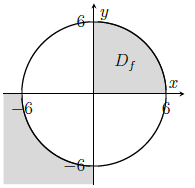
\includegraphics[scale=0.6]{pictures/3_4_a}
	\end{center}
	\item 
	\begin{center}
		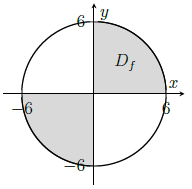
\includegraphics[scale=0.6]{pictures/3_4_b}
	\end{center}
	\item
	\begin{center}
		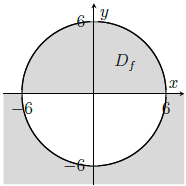
\includegraphics[scale=0.6]{pictures/3_4_c}
	\end{center}
	\item
	\begin{center}
		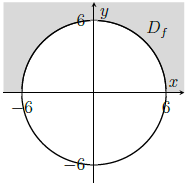
\includegraphics[scale=0.6]{pictures/3_4_d}
	\end{center}
\end{enumerate}
\ \\
\textbf{Lösung:}
\begin{mdframed}
\underline{\textbf{Vorgehensweise:}}
\renewcommand{\labelenumi}{\theenumi.}
\begin{enumerate}
\item Bestimme den Definitionsbereich.

\end{enumerate}
\end{mdframed}

\underline{1. Bestimme den Definitionsbereich}\\
Für den Term unter der Wurzel muss $ (36 - x^2 -y^2) y \geq  0 $ gelten.
Hierfür betrachten wir zwei Fälle:
\begin{description}
	\item[1. Fall $ y \geq 0 $:] 
	Wir können $ y > 0  $ annehmen, denn $ y = 0 $ ist uninteressant.
	Damit gilt:
	\begin{align*}
		(36 - x^2 -y^2) y  \geq   0
		\ \Leftrightarrow \ 
		36 - x^2 -y^2   \geq   0
		\ \Leftrightarrow \ 
		x^2 +y^2 \leq 36 = 6^2.
	\end{align*}
	Für $ y > 0  $ erhalten wir eine Kreisscheibe mit Radius $ 6 $.
	
	\item[2. Fall $ y < 0 $:] 
	Für $ y <0  $ gilt:
	\begin{align*}
		(36 - x^2 -y^2) y  \geq   0
		\ \Leftrightarrow \
		(36 - x^2 -y^2) \leq 0
		\ \Leftrightarrow \
		x^2 + y^2 \geq 36 = 6^2.
	\end{align*}
	Somit erhalten wir in diesem Fall den Bereich auf und außerhalb des Kreises mit Radius $ 6 $.
\end{description}
Damit ist Antwort (c) korrekt.
\newpage

\subsection*{\frage{5}{3}}
Welche der folgenden Funktionen gehört zur unten dargestellten Fläche?\\
\begin{center}
	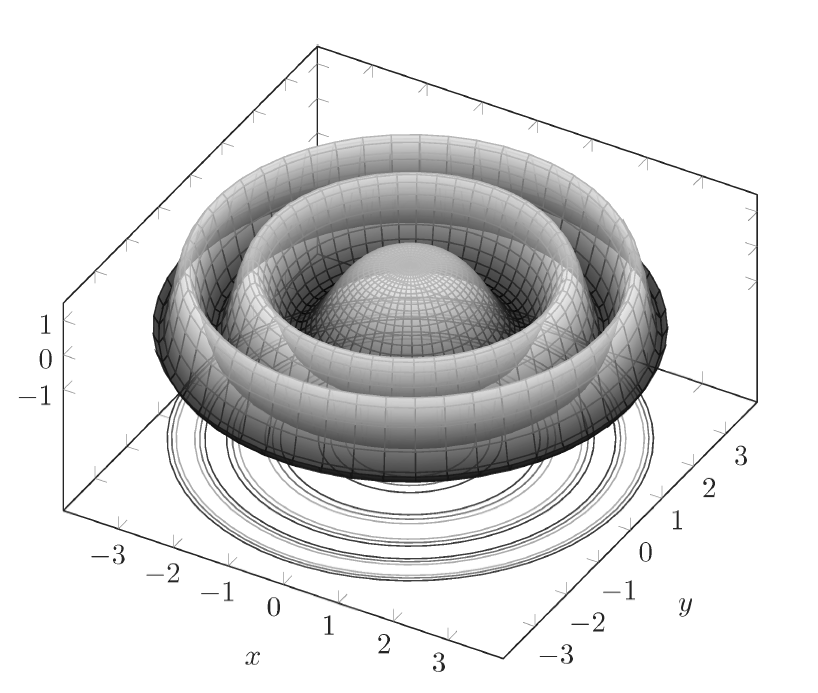
\includegraphics[scale=0.5]{pictures/3_5}
\end{center}
\renewcommand{\labelenumi}{(\alph{enumi})}
\begin{enumerate}
	\item 
	$ z = f_1(x,y) = e^{-(x+y^2)} $.
	\item
	$ z = f_2(x,y) = e^{x} e^y $.
	\item
	$ z = f_3(x,y) = e^{2 -x^2 +y^2}  $.
	\item
	$ z = f_4(x,y) = \cos(x^2 +y^2) $.
	\item
	$ z = f_5(x,y) = 2^{-(x + y^2)} $.
	\item
	$ z = f_6(x,y) = \sin(x+y) $.
\end{enumerate}
\ \\
\textbf{Lösung:}
\begin{mdframed}
\underline{\textbf{Vorgehensweise:}}
\renewcommand{\labelenumi}{\theenumi.}
\begin{enumerate}
\item Schränke die Antwortmöglichkeiten ein.
\item Bestimme die korrekte Antwort.
\end{enumerate}
\end{mdframed}

\underline{1. Schränke die Antwortmöglichkeiten ein}\\
Die Grafik zeigt deutlich, dass sich der Wertebereich zwischen $ -1 $ und $ 1 $ bewegt. Der Wert an $ (0,0) $ ist $ 1 $.
Damit können wir die Antworten (c) und (f) ausschließen.
Weiter gilt:
\begin{align*}
	\lim \limits_{x \to -\infty}
	f_1(x,0) 
	&=
	\lim \limits_{x \to -\infty} e^{-(x +0^2)} 
	= 
	\lim \limits_{x \to -\infty} e^{-x} = \infty\\
	\lim \limits_{x \to \infty}
	f_2(x,0) 
	&=
	\lim \limits_{x \to \infty}
	e^x e^0 
	=
	\lim \limits_{x \to \infty}
	e^x 1 
	=
	\infty\\
		\lim \limits_{x \to -\infty}
	f_5(x,0) 
	&=
	\lim \limits_{x \to -\infty} 2^{-(x +0^2)} 
	= 
	\lim \limits_{x \to -\infty} 2^{-x} = \infty
\end{align*}
Da die Funktionen unbeschränkt sind, kann der Wertebereich nicht zwischen $ -1 $ und $ 1 $ liegen.
Somit sind die Antworten (a),(b) und (e) falsch. Also bleibt die Antwort (d) übrig.\\
\\
Damit ist Antwort (d) korrekt.
\\
\\
Alternativ kann man sich überlegen, welche Funktionen Kreise als Niveaulinien haben.


\newpage

\subsection*{\frage{6}{4}}
Wir betrachten die Cobb-Douglas Produktionsfunktion
\begin{align*}
	P(K,A) 
	=
	4 K^{0.25} A^{0.75} \ \ (K,A > 0).
\end{align*}
Für welchen Punkt $ (K_0, A_0) $ auf der Isoquante (Niveaulinie) $ P(K,A) = 64 $ ist die technische Substitutionsrate (des Faktors Arbeit $ A $ bezüglich des Faktors $ K $) gleich $ - \frac{1}{3} $ ?
\renewcommand{\labelenumi}{(\alph{enumi})}
\begin{enumerate}
	\item 
	$ (K_0, A_0) = ( 8 \sqrt{2}, 8 ) $.
	\item
	$ (K_0, A_0) = ( 8 , 16 )$.
	\item
	$ (K_0, A_0) = ( 32 , 32)$.
	\item
	$ (K_0, A_0) = ( 4 , 4\sqrt{2})$.
	\item
	$ (K_0, A_0) = ( 16 , 16\sqrt{2})$.
	\item
	$ (K_0, A_0) = ( 16 , 16)$.
\end{enumerate}
\ \\
\textbf{Lösung:}
\begin{mdframed}
\underline{\textbf{Vorgehensweise:}}
\renewcommand{\labelenumi}{\theenumi.}
\begin{enumerate}
\item Bestimme die technische Substitutionsrate.
\end{enumerate}
\end{mdframed}

\underline{1. Bestimme die technische Substitutionsrate}\\
Die technische Substitutionsrate ist gegeben durch:
\begin{align*}
	T(A,K) = - \frac{P_K(K,A)}{P_A(K,A)}
	 = -\frac{4 \cdot 0.25 \cdot K^{-0.75} A^{0.75}}{4 \cdot 0.75 \cdot  K^{0.25} A^{-0.25}} 
	 =
	 -\frac{A}{3 K }. 
\end{align*}
Für die Niveaulinie $ P(K,A) = 64  $ soll $ T(A,K) = -\frac{1}{3} $ gelten. Hierfür lösen wir zunächst $ P(K,A) = 64  $ nach $ K $ auf:
\begin{align*}
	P(K,A )= 4 K^{0.25} A^{0.75} = 64 
	\ \Leftrightarrow \
	K^{0.25} = \frac{64}{4 A^{0.75}}
	= \frac{16}{A^{0.75}}
	\ \Leftrightarrow \
	K = \frac{16^4}{A^3}. 
\end{align*}
Eingesetzt in die technische Substitionsrate ergibt dies:
\begin{align*}
	T(A,K)
	=
	-\frac{A}{3 K }
	=
	- \frac{A}{3 \frac{16^4}{A^3}}
	=
	- \frac{A^4}{3 \cdot 16^4}
	=
	- \frac{1}{3}
	\ \Leftrightarrow \
	A = 16.
\end{align*}
Damit gilt auch 
\begin{align*}
	K = \frac{16^4}{16^3} = 16.
\end{align*}
Somit ist die technische Substitutionsrate für $ (16,16) $ gleich $ - \frac{1}{3} $ (Auf der Niveaulinie $ P(K,A ) = 64 $).\\
\\
Also ist Antwort (f) korrekt.




\newpage



\subsection*{\frage{7}{3}}
Gegeben ist die Funktion
\begin{align*}
	f(x,y) 
	=
	x^2 e^{\frac{x+y}{x}}
	-
	xy e^{\frac{x+y}{x-y}}
	+
	x \ln \left( \frac{x}{y} \right)
	\quad \textrm{für } x>0,y>0.
\end{align*}
Welche der folgenden Aussagen ist richtig?
\renewcommand{\labelenumi}{(\alph{enumi})}
\begin{enumerate}
	\item
	$ f  $ ist homogen vom Grad $ 0 $.
	\item
	$ f  $ ist homogen vom Grad $ 0.5 $.
	\item
	$ f $ ist linear homogen.	
	\item 
	$ f  $ ist homogen vom Grad $ 2 $.
	\item
	$ f $ ist nicht homogen.
\end{enumerate}
\ \\
\textbf{Lösung:}
\begin{mdframed}
\underline{\textbf{Vorgehensweise:}}
\renewcommand{\labelenumi}{\theenumi.}
\begin{enumerate}
\item Überlege, ob $ f $ homogen sein kann.
\end{enumerate}
\end{mdframed}

\underline{1. Überlege, ob $ f $ homogen sein kann}\\
Wir betrachten die einzelnen Summanden von $ f $ und untersuchen diese auf Homogenität:
\begin{align*}
	f_1(x,y)
	&=
	x^2 e^{\frac{x+y}{x}}\\
	f_2(x,y)
	&=
	-
	xy e^{\frac{x+y}{x-y}}\\
	f_3(x,y)
	&=
	x \ln \left( \frac{x}{y} \right).
\end{align*} 
Wir untersuchen nun jeweils die Homogenität.
Sei $ \lambda \in \R $ beliebig. Dann gilt:
\begin{align*}
	f_1(\lambda x, \lambda y)
	&=
	(\lambda x)^2 e^{\frac{\lambda x+ \lambda y} { \lambda x}}
	=
	\lambda^2 x^2 e^{\frac{\lambda( x+  y) } { \lambda x}}
	=
	\lambda^2 x^2 e^{\frac{x+y}{x}} 
	= \lambda^2 f_1(x,y)
	\\
	f_2(\lambda x, \lambda y)
	&=
	-
	\lambda x \lambda y e^{\frac{\lambda x+ \lambda y}{ \lambda x- \lambda y}}
	=
	-
	\lambda^2 xy e^{\frac{\lambda (x+  y)}{ \lambda (x-  y)}}
	=
	-
	\lambda^2 xy e^{\frac{x+  y}{  x-  y}}
	=
	\lambda^2 f_2(x,y)\\
	f_3(\lambda x, \lambda y)
	&=
	\lambda x \ln \left( \frac{\lambda x}{ \lambda y} \right)
	=
	\lambda x \ln \left( \frac{ x}{ y} \right)
	=
	\lambda f_3(x,y).
\end{align*}
Damit sind die ersten beiden Summanden homogen vom Grad $ 2 $.
Der dritte Summand ist homogen vom Grad $ 1 $. Aufgrund des Distributivgesetz müssten alle Summanden von $ f $ dieselbe Homogenität besitzen, damit $ f $ homogen ist. Also ist $ f $ nicht homogen.\\
\\
Damit ist Antwort (e) korrekt.


\newpage

\subsection*{\frage{8}{4}}
Gegeben ist die Funktion
\begin{align*}
	f(x,y)
	=
	\frac{x^{2a} y^b}{x^3 +y^3}
	- 
	\frac{1}{x^3 y^{3b} + x y^{2 + 3b}},
\end{align*}
wobei $ x > 0, y > 0 $ und $ a,b \in \R $.\\
\\
Für welche Werte von $ a $ und $ b $ gilt
\begin{align*}
	x f_x(x,y) + y f_y(x,y) = 0 \ \textrm{für alle } x>0, y>0\textrm{?}
\end{align*}
\renewcommand{\labelenumi}{(\alph{enumi})}
\begin{enumerate}
	\item 
	$a = 2$ und $ b=-1 $.
	\item
	$a = 1$ und $ b=1 $.
	\item
	$a = 1$ und $ b=-1 $.
	\item
	$a = 3$ und $ b=-2 $.
	\item
	$a = -2$ und $ b=1 $.
	\item
	Es gibt keine Werte $ a $ und $ b $, die die Bedingung erfüllen.
\end{enumerate}
\ \\
\textbf{Lösung:}
\begin{mdframed}
\underline{\textbf{Vorgehensweise:}}
\renewcommand{\labelenumi}{\theenumi.}
\begin{enumerate}
\item Verwende die Eulersche Relation.
\end{enumerate}
\end{mdframed}

\underline{1. Verwende die Eulersche Relation}\\
Falls $ f $ homogen vom Grad $ \kappa $ ist, besagt die Eulersche Relation
\begin{align*}
	\varepsilon_{f,x}(x,y) + \varepsilon_{f,y}(x,y) 
	= x \frac{f_x(x,y)}{f(x,y)} + y \frac{f_y(x,y)}{f(x,y)}
	= \kappa.
\end{align*}
Dies ist äquivalent zu:
\begin{align*}
	x f_x(x,y) + f_y(x,y) = \kappa \cdot f(x,y).
\end{align*}
Wie müssen nun überprüfen, für welche $ a, b\in \R $ eine Homogenität von $ 0 $ vorliegt:
\begin{align*}
	f(\lambda x, \lambda x)
	&=
	\frac{(\lambda x)^{2a} (\lambda y)^b}{(\lambda x)^3 +(\lambda y)^3}
	- 
	\frac{1}{(\lambda x)^3 (\lambda y)^{3b} + (\lambda x) (\lambda y)^{2 + 3b}}
	=
	\frac{\lambda^{2a +b} ( x^{2a}  y^b)}{\lambda^3 (x^3 + y^3 )}
	- 
	\frac{1}{\lambda^{3b + 3} x^3  y^{3b} + \lambda^{3b + 3} x  y^{2 + 3b}}\\
	&=
	\frac{\lambda^{2a +b}}{\lambda^3}\frac{ ( x^{2a}  y^b)}{ (x^3 + y^3 )}
	- 
	\frac{1}{\lambda^{3b + 3}}\frac{1}{ x^3  y^{3b} +  x  y^{2 + 3b}}
	=
		\lambda^{2a +b - 3}\frac{ ( x^{2a}  y^b)}{ (x^3 + y^3 )}
	- 
	\lambda^{-(3b + 3)}\frac{1}{ x^3  y^{3b} +  x  y^{2 + 3b}}.
\end{align*}
Damit $ f $ homogen vom Grad $ 0 $ ist, muss 
\begin{align*}
	2a + b - 3 &= 0\\
	-3b - 3 &= 0
\end{align*}
gelten. Für die zweite Gleichung gilt:
\begin{align*}
	-3b - 3 = 0 
	\ \Leftrightarrow \
	-3b = 3
	\ \Leftrightarrow \
	b = -1.
\end{align*}
Wenn wir dies in die erste Gleichung einsetzen, erhalten wir:
\begin{align*}
	2a - 1 - 3 = 0 
	\ \Leftrightarrow \
	2a = 4
	\ \Leftrightarrow \
	a = 2.
\end{align*}
Somit ist $ f $ für $ a = 2 $ und $ b= -1 $ homogen vom Grad $ 0 $ und die erwünschte Gleichung ist erfüllt.\\
\\
Also ist Antwort (a) korrekt.


